\chapter{Internal Electrode Motion}
\label{chap:chapter-7}

\emph{Preliminary animal reconstructions have
 been presented in part at: 
 the 21st International Conference on Biomedical 
 Applications of Electrical Impedance Tomography (EIT 2021)~\parencite{stowe_using_2021}.} 

\section{Introduction}
Internal electrode have been shown several times to improve sensitivity in the internal regions 
of a model, and improve reconstruction accuracy
\parencite{nasehi_tehrani_modelling_2012,nasehi_tehrani_evaluation_2012,nguyen_electrical_2020,pilkington_utilization_1989,schuessler_utility_1995}.
When used in a clinical setting they have shown an increase in sensitivity to cardiosynchronous
EIT signals in most subjects \parencite{czaplik_application_2014}, but they have not been widely used 
in real-world settings. 
Image reconstructions using internal electrodes are challenging and have not yet 
been used consistently \emph{in-vivo}.
One of the main factors that may contribe to confounding real-world EIT recordings is movment 
of the internal probe. 
It is not clear how much changes in location between the probe impact EIT measurements.
Typically when reconstructing EIT images, using difference imaging reduces the impact of 
systematic errors, but electrodes on an internal probe can move quickly and may change location 
during measurements. 
The effect of this electrode motion is not well understood and currently no analysis exists 
that explores the effect of internal probe movment on reconstructed images. 
\parencite{nguyen_review_2012}. 
This chapter presents an analysis of the impact of internal probe movement on 
EIT reconstructions using internal electrodes, and introduces a technique to correct for probe 
movement that is up to 10\% of the model radius.

As discussed in \fref{sec:bioimpedance}, several factors contribute towards
the cardiosynchronous signal in EIT. One of the largest contributions 
is movement; both the movement of 
body structures and the movement of electrodes contribute significantly to the measured
impedance and the resulting reconstructed 
image~\parencite{adler_origins_2017,proenca_influence_2015}.
The previous chapters support that more accurate meshing and internal electrodes may
help to identify the movement of structures and organs, and isolate their impact on
reconstructed images, but the problem of electrode motion is amplified when internal
electrodes are used. 
Internal electrodes placed on a probe are challenging to locate within a subject
due to variation in individual geometries. Incorrectly modelling the electrode 
locations can introduce an artefact in the image~\parencite{boyle_impact_2011}, 
but in time difference EIT these effects are reduced~\parencite{adler_electrical_2017}. 
The larger problem appears 
to be the 
movement of the internal probe relative to the external electrodes between
measurements. Recent work by~\citeauthorandyear{nguyen_electrical_2020}
reviewed the potential aplication of internal electrodes in cardio 
radiofrequency ablation and discussed the need for an analysis 
of the effect of heart motion on the internal electrode, and a solution 
to correct for its impact on EIT reconstructions.

Movement correction algorithms using the movement jacobian have been 
designed in 2D 
and 3D~\parencite{gomez-laberge_direct_2007,soleimani_imaging_2006,gomez-laberge_direct_2008}
and used to reconstruct electrode movement on 3D models with a 2D arrangement 
of electrodes~\parencite{boyle_geophysical_2016}. 
There are several available methods to calculate the movement 
jacobian~\parencite{boyle_methods_2017}. The simplest of which,
the na\"{i}ve perturbation method~\parencite{gomez-laberge_direct_2008},
has been used in this chapter as a proof of concept.  
A more detailed explanation of this jacobian calculation method is presented in 
\fref{sec:motion_correction} of the background.
As an internal probe moves towards one side of a model the distance between the 
probe and the external electrodes changes. This results in lower 
impedance where the distance 
has decreased, and a higher impedance where the distance has increased. Without knowing 
the new probe location we can reduce the effect of this error, but there still remains 
a mismatch between the modelled and actual probe locations. 
The artefact that is reconstructed can give hints regarding the motion of electrodes,
although it can be difficult to separate the effect of electrode movement 
from biological impedance changes of interest~\parencite{boyle_geophysical_2016}. 

This chapter presents a method that builds on currently available
algorithms, to create a new, corrected model
that helps to compensate for the effect of electrode movement.  
The known shape of the artefact due to movement of the probe is used to 
derive the probe location, and create a corrected model to improve 
reconstruction accuracy in the presence of probe motion.

The goal of this chapter is to develop and validate a technique to reduce the impact of probe movement on 
image reconstructions, and then to test this technique in an animal model. 
Although simulations in 2D, and now in 3D, show that internal electrodes can provide 
a desirable increase in sensitivity, the benefit has not been realized in real-world
recordings. 
The relatively large amount of promosing simulation work compared to limited real-world 
results suggest that this is a challening problem. 
It has been suggested that error due to electrode motion may be a major contributing 
factor to the the EIT signal on internal electrodes \parencite{nguyen_electrical_2020},
and we believe this may be one of the largest sources of error in real-world 
EIT measurements. 
In this chapter we investigate the impact of motion on internal electrode EIT and explore 
techniques to solve this problem and reconstruct images in the presence of electrode motion.
This chapter presents a novel method to correct for electrode displacement artefacts, and evaluates 
how it is able to minimize electrode motion errors.
This new technique is compared to 
established techniques for 3D EIT image reconstruction 
to reconstructions on a limited number of 
subjects in an animal model.

\section{Methods}
This chapter describes the analysis for both: a simulation study correcting for probe motion 
in a tank model, and preliminary \emph{in-vivo} recordings that were conducted 
in conjunction with a larger experimental protocol. 

\subsection{Simulations}
To model electrode motion measure the effect on reconstruction accuracy simulations 
in a tank model were used.
Simulations were done using EIDORS (v3.10)~\parencite{adler_eidors_2017}
using Matlab 2019b (Matworks, Natick, MA, USA).
Within EIDORS, meshes were generated using 
Netgen (version 5.3.1)~\parencite{schoberl_netgen_1997}.

\subsubsection{Tank models}
On a tank model 28 external electrodes were placed in two planes of 14. 
4 internal electrodes were placed evenly between the top and bottom external electrode planes. 
The tank radius and height were 1 m, and the external electrode radius was 5 cm. 
The external electrode planes were placed at a height of 0.3 m and 0.7 m on the tank. 
The internal electrodes were spaced evenly between the external electrode planes 
at 0.3 m, 0.433 m, 0.567 m and 0.7 m. The internal electrodes were specified in 
two different ways. The first used spheres with a radius of 2.5 cm, and the second 
used a hollow cylinder with a radius of 2.5 cm containing cylindrical electrodes
with a radius of 2.5 cm and a height of 5 cm. External electrodes were
placed in a ``square'' electrode configuration~\parencite{grychtol_3d_2016}. 
Both models are shown in \fref{fig:probe_types}.

\begin{figure}
    \centering
   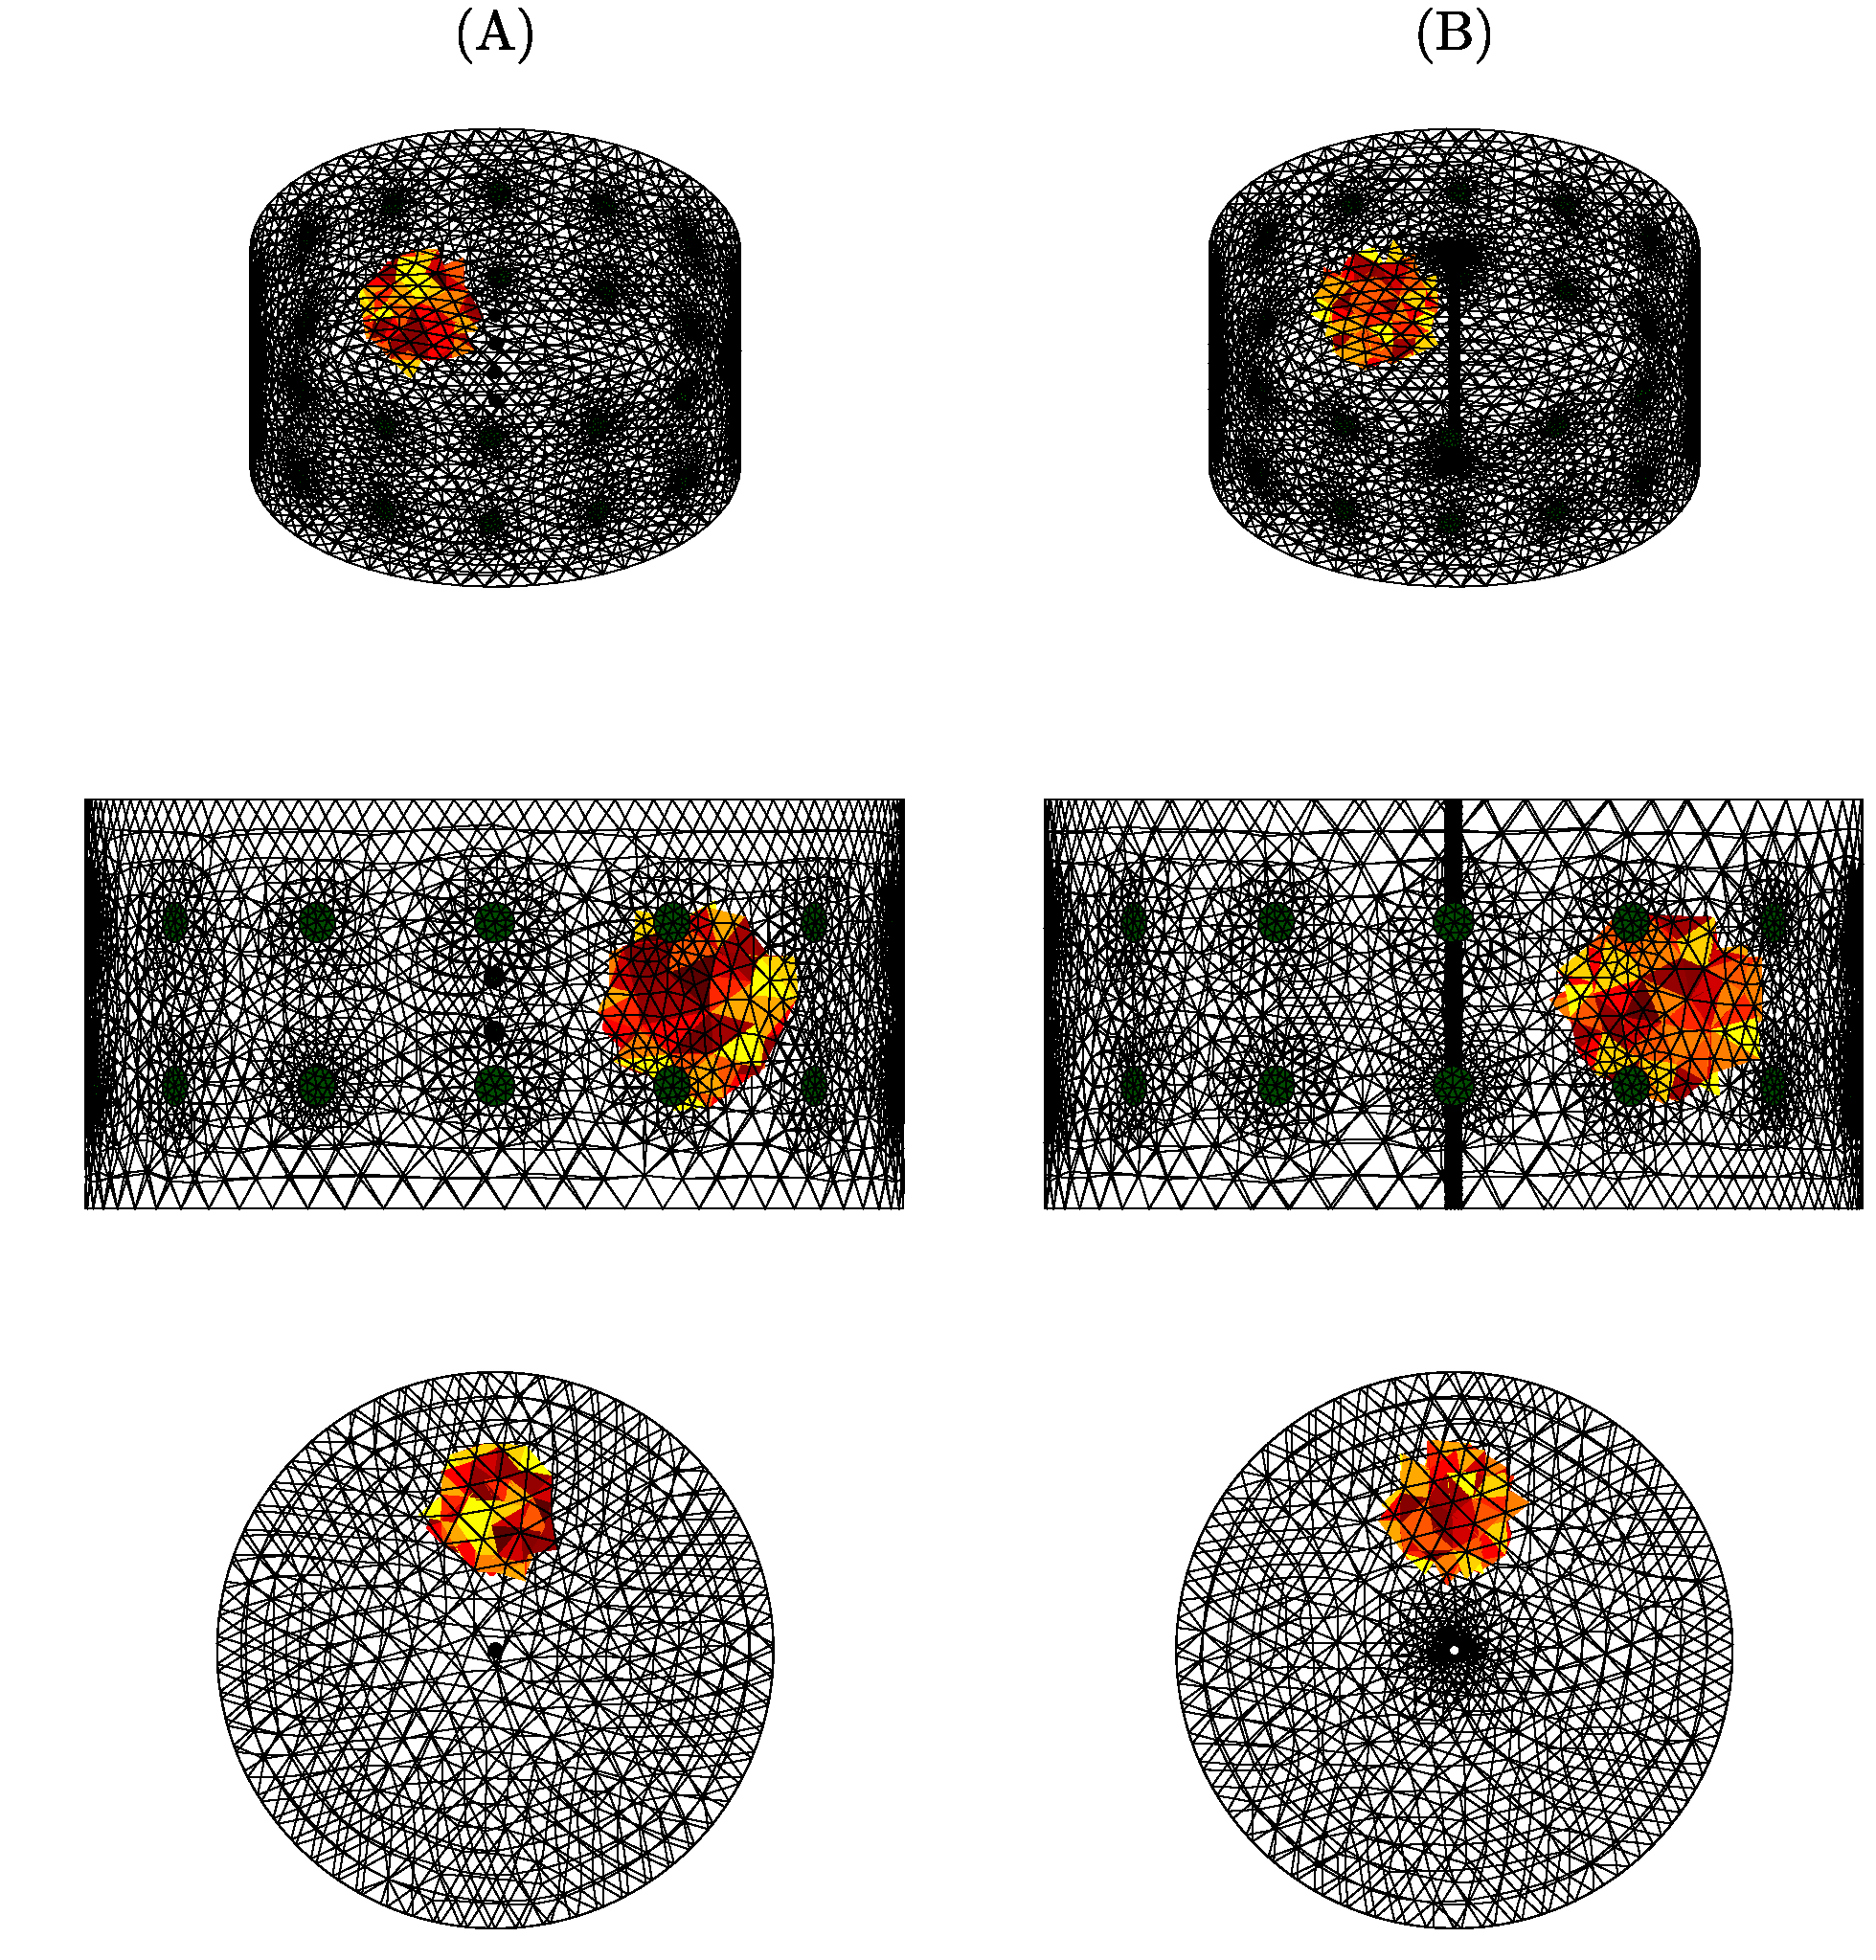
\includegraphics[width=\textwidth]{chapter7-internal_elec_motion/imgs/probe_types.pdf} 
   \caption[Spherical and cylindrical internal electrodes]{\label{fig:probe_types} 
   On the left (A) internal electrodes were modelled as 4 spherical electrodes between the 
   external electrode planes. On the right (B) the internal electrodes were created using 
   a hole through the centre of the model and using cylindrical electrodes on the inner 
   surface of the model.
	The conductive region was specified by setting the conductivity of all elements 
	contained in the target to be twice the background conductivity.}
\end{figure}

These models were compared to verify that both 
performed adequately with motion correction, as internal electrodes 
are challenging to model and many different techniques are used. 
When using internal electrodes on a complex model, it is currently easiest 
to add electrodes along a hollow tube cut through the centre, since 
a small circle can be specified in EIDORS functions that are designed to make extruded 
models. This circle when extruded up with the boundary will form a small hole representing 
the probe where electrodes can be placed.

To specify a conductive region, elements within a radius were assigned a conductivity 
of twice the background conductivity of the tank model.
The conductive target was placed midway between the centre of the tank and the boundary. 
The radius of the target was 20 cm. 
\Fref{fig:probe_types} shows the conductive target for both internal probe types.

\subsubsection{Measurements}
The skip 4 currnet injection and measuremnt pattern was used as it can be 
easily implemented on most EIT systems, and was shown to have a very even 
sensitivity distribution in 3D EIT \parencite{grychtol_3d_2016}.
%Despite sensitivity advantages ascribed to custom injection and 
%measurement patterns, the skip 4 pattern was used as it 
%is straight forward to implement with currently available EIT systems. 

Reference measurements were made with no conductive object and 
electrodes in the centre of the model. Measurements with a conductive object were made 
with the probe centred, then
with the probe was shifted by 1, 5, and 10 percent of the tank radius in a randomized 
direction. The direction was randomized between trials but was consistent for 
each of the 1, 5 and 10 percent probe error models that were compared. 

\subsection{Movement correction}
\label{sec:3_methods}

As shown in \fref{sec:inv_prob}, the jacobian in typical EIT reconstruction 
represents the sensitivity of the voltage measurements to a change in conductivity. 
In this chapter we will refer to this as the conductivity jacobian ($J_C$). 
A similar formulation can be used for the movment, but instead of the sensitivity 
to change in conductivity, we want the jacobian to represent the 
change in measured voltage 
sensitivity due to movement of the probe. to calculate the movement jacobian we can use:
\begin{equation}
	[J_M]_l = \frac{\Delta\mathbf{V}_l}{\Delta\mathbf{r}_l},
\end{equation}
where $\mathbf{r}$ is the change in position of an electrode $l$.
The movement jacobian is a derivative of the measurements with respect to the movement.
To aproximate the movement derivative we can use a perturbation to 
shift each electrode by a small amount (0.001 m), and calculating the 
change in voltage measurements \parencite{gomez-laberge_direct_2008}.

The movement correction jacobian was calculated using the methods presented by
\citeauthorandyear{gomez-laberge_direct_2008}. In a model with a centred electrode
probe and uniform conductivity, each of the four electrodes on the probe was
perturbed by 0.001 m in each of the $\mathbf x$, $\mathbf y$, 
and $\mathbf z$ directions. A measurement was made for 
each electrode and each of the three dimensions of movement. 
The resulting measurements were divided by the perturbation 
amount. 
The measurements on each electrode ($V_j$) and from each  direction 
of movement ($\mathbf x$, $\mathbf y$, 
and $\mathbf z$) were combined to form the movement 
jacobian ($J_M$) using the following equation from
\citeauthorandyear{gomez-laberge_direct_2008}:
\begin{equation}
	J_M = \left[ 
		  \frac{\partial\mathbf{V}_j}{\partial\mathbf{x}},
		  \frac{\partial\mathbf{V}_j}{\partial\mathbf{y}},
	      \frac{\partial\mathbf{V}_j}{\partial\mathbf{z}} ... 
		  \frac{\partial\mathbf{V}_n}{\partial\mathbf{x}},
		  \frac{\partial\mathbf{V}_n}{\partial\mathbf{y}},
	      \frac{\partial\mathbf{V}_n}{\partial\mathbf{z}} 
		  \right]
\end{equation}

This movement jacobian was used in conjunction with the following single-step 
formulation for a reconstruction matrix presented 
by \citeauthorandyear{adler_impedance_1994}. The regular impedance-based 
reconstruction matrix is denoted by $R_C$ and the jacobian for impedance-based 
reconstruction is denoted by $J_C$.
\begin{equation}\label{eq:regular_rm}
	R_C = [J_C]^T [W]\left([J_C] [W] [J_C]^T + [W]\right)^{-1}
\end{equation}
$W$ in the above equation represents the Laplace prior~\parencite{soleimani_imaging_2006}.
Combining this formulation with the movement jacobian yields the following equation 
for the reconstruction matrix ($R_M$)~\parencite{soleimani_imaging_2006}, where $R_M$
denotes the reconstruction matrix for motion correction.
\begin{equation}\label{eq:motion_rm}
	R_M = [J_C]^T [W]([J_C] [W] [J_C]^T + \mu [J_M][J_M]^T + [W])^{-1}
\end{equation}
In the above equation $\mu$ represents the weighting of the motion correction. 
In this experiment the motion correction weighting was set to 100. 

Combining \fref{eq:regular_rm} and \fref{eq:motion_rm}, a reconstruction
matrix to reconstruct exclusively the noise due to movement ($R_N$) 
in an image can be generated.
\begin{equation} \label{eq:noise_rm}
	R_N = R_M - R_C
\end{equation}

%$R_N$ can also be calculated directly by combining \fref{eq:regular_rm}
%and \fref{eq:motion_rm}. 
%

An image ($X$) is reconstructed using 
the measurements ($b$) and reconstruction matrix ($R$) as follows:

\begin{equation}
	X = bR
\end{equation}

Three images: $X_C$, $X_M$ and $X_N$ were reconstructed from their 
respective reconstruction matrix. 

A new movement correction strategy had been built 
around the reconstructed image $X_N$.
As a probe is moved towards electrodes on the the edge of the model 
conductivity is decreased and this is shown as a conductive object in the reconstructed 
image. Using $R_N$ we are able to reconstruct the 
size and shape of the artefact due to only electrode motion,
and determine the approximate direction and amplitude of
the probe movement.
In the reconstructed image 
showing only the motion artefact,
the centre of mass of the positive change is located. 
This is assumed to be the direction of the motion. The amplitude of the electrode 
motion is estimated as half of the distance between the 
conductive artefact and the probe. This method is illustrated in
\fref{fig:motion_correction_methods}. Images were reconstructed and displayed 
on a 64 by 64 grid to give a more accurate representation of the 
electrode position in the reconstructed image.

\begin{figure}
    \centering
   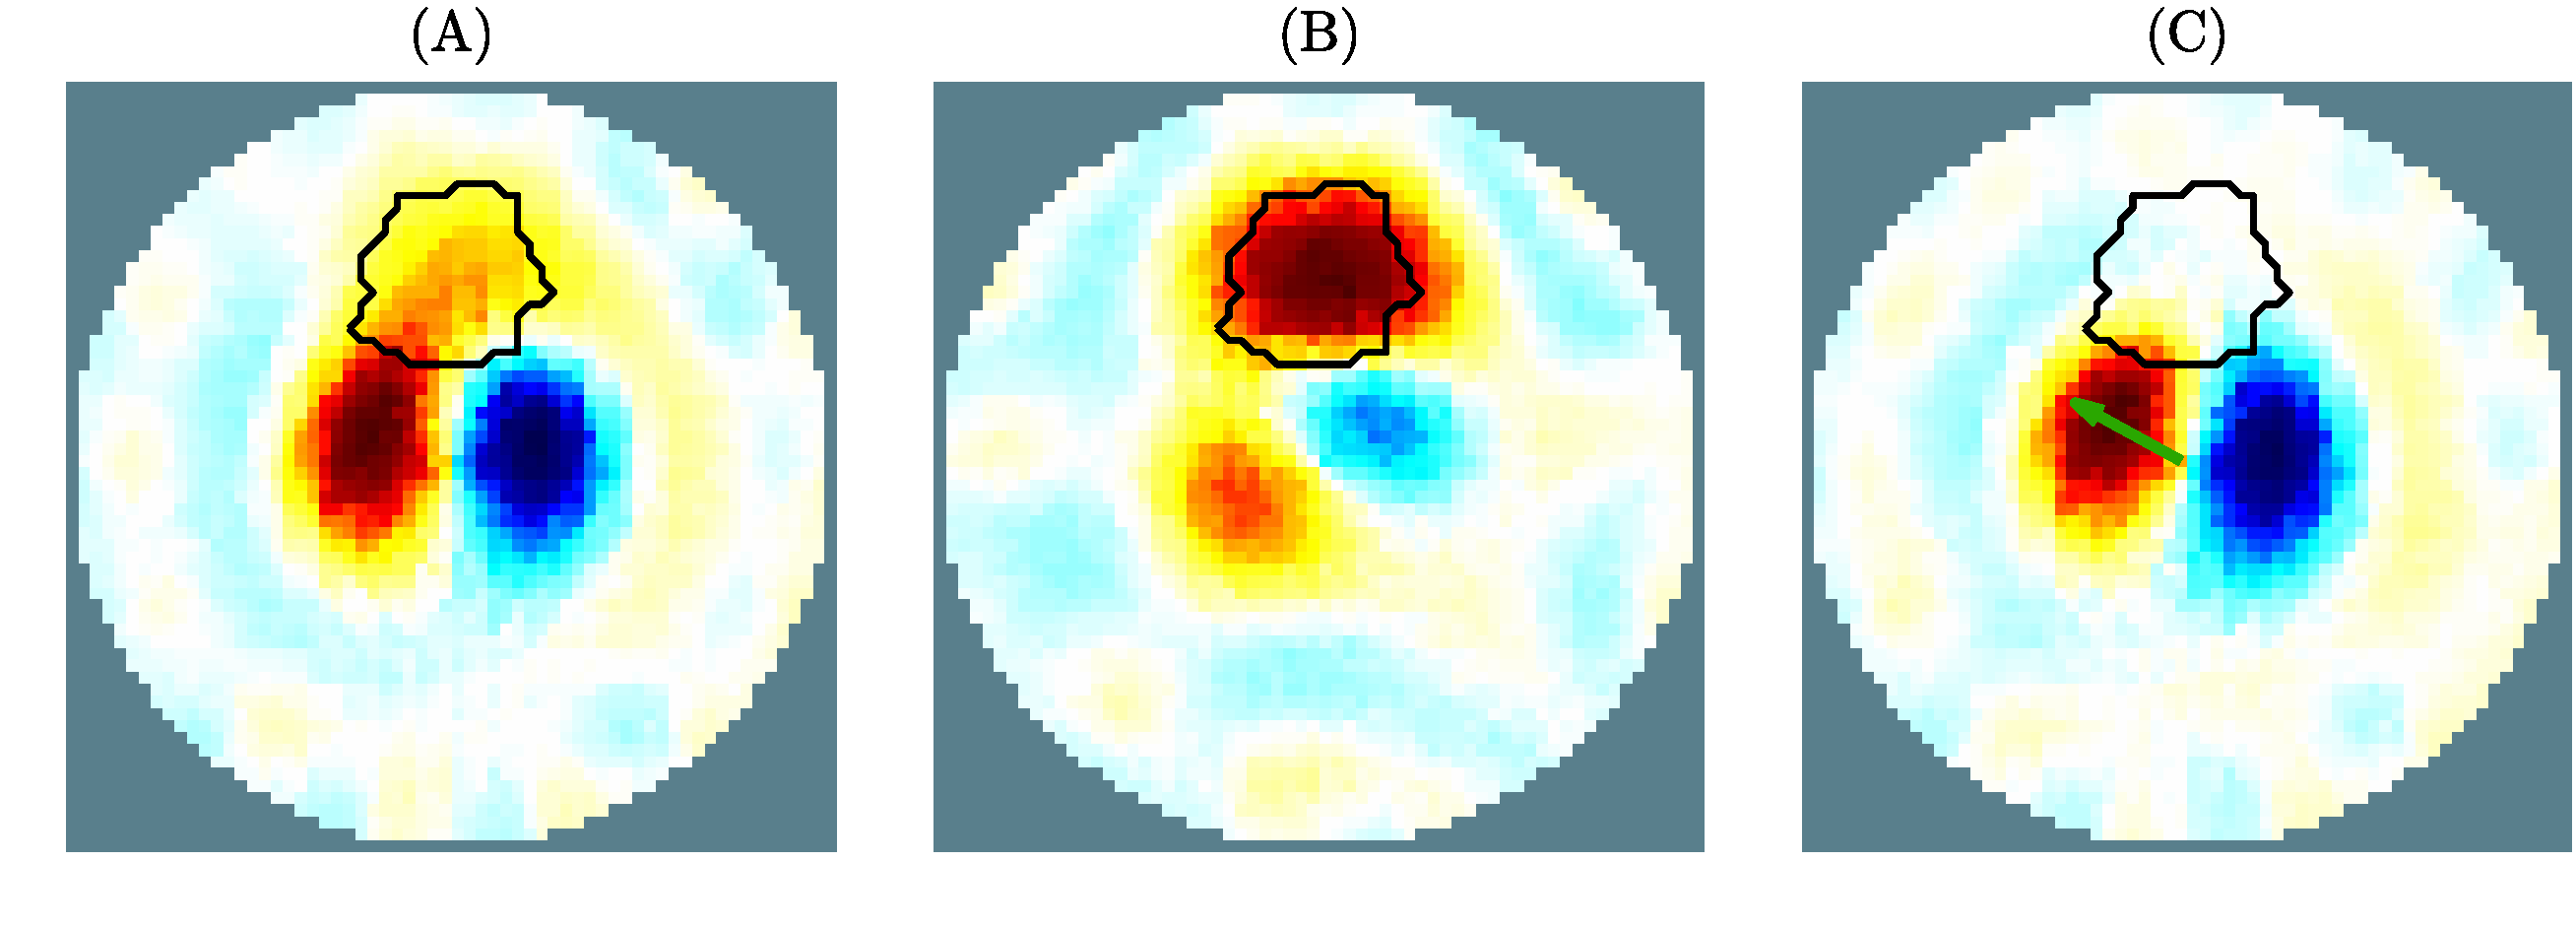
\includegraphics[width=\textwidth]{chapter7-internal_elec_motion/imgs/recon_methods.pdf} 
   \caption[Motion correction methods]{\label{fig:motion_correction_methods} 
   This figure shows the 3 scenarios of the initial image reconstruciton. 
   Image (A) shows the image reconstructed using the typical conductivity jacobian 
   from \fref{eq:regular_rm}. Image (B) shows the image reconstruced using the movment 
   jacobian ans equation \fref{eq:motion_rm}. Finally image (C) shows the 
   isolated image artefact reconstructed using the reconstruction matrix in 
   \fref{eq:noise_rm}
	The centre of mass of the conductive object in (C) is used to
	estimate the probe location and direction of movement. The green arrow indicates the 
	calculated direction of movement (multiplied by 5 for visibility).
	The black line indicates the outline of the region of conductivity at the imaged plane.
	The images depict an average of 10 slices between the external electrode planes.}
\end{figure}

Using the probe location estimate calculated from $X_N$,
a new model was reconstructed with the probe repositioned 
to the reconstructed location. 
This model was then used to calculate a new reconstruction matrix 
using \fref{eq:motion_rm}
with an updated jacobian based on the new probe location. 


\subsection{Image comparison}
To simplify processing of the reconstructions, 10 images between the 
external electrode planes were averaged together to generate a 2D 
representation of the 3D data. This did not allow for analysis of movement in the vertical 
direction, but we did not expect this to be a major contribution in real-world data.
The reconstructed images were compared in two ways. First, the accuracy of the reconstruction
was evaluated by computing the Jaccard index \parencite{jaccard_distribution_1912} 
between the actual and imaged boundaries of the 
conductive target. The imaged boundary was drawn at half the maximum value of the brightest 
object in the image. The second metric computed was a noise estimate. This was calculated as
the amplitude of the imaged object relative to the amplitude of the entire image through the
following equation:

\begin{equation}
	N = 1-\frac{A_{\text{object}}}{A_{\text{image}}}
\end{equation}

Where $A_{\text{object}}$ is the amplitude of the object, $A_{\text{image}}$ is the amplitude 
of the image, and the ratio is subtracted from 1 so that a noise estimate 
of 0 corresponds with 
all of the image signal originating from the conductive target.

\subsection{\emph{In-vivo} recordings}
This experiment was approved as an amendment to an existing protocol (2018-2131) 
by the Université de Sherbrooke Ethics Board. The pregnant ewe carrying two lambs was 
premedicated using an intramuscular injection of 10 mg/kg of ketamine and intubated. 
Anesthesia was maintained using 2--4 \% isoflurane in conjunction with conventional 
mechanical ventilation (CMV). Lambs were birthed prematurely at 120 days of 
gestation (147 days normal gestation) through caesarean section. 
One lamb was ventilated with either CMV or total liquid ventilation (TLV) for 6 hours. 
The other lamb served as a paired control to assess 
lung and cerebral inflammation resulting from ventilation. 

Data were collected in three ewes during CMV 
using the SenTec EIT Pioneer Set.
A skip 4 measurement pattern was used with an injection current 
of 3 mA at 30 kHz. Electrodes 29 to 32 were connected to the internal
electrode probe. 

\subsubsection{Internal electrode probe design}
The internal electrode probe consisted of four brass electrodes on a flexible tube. 
Each electrode was 1 cm in length and the spacing between electrodes was 2 cm. 
The electrodes were created from
a brass sheet with a thickness of 2 mm that was bent to the shape 
of the flexible tubing and soldered to 
achieve a smooth surface. The electrodes were glued in place 
on the tube, protruding 2 mm from probe surface.
The tube radius was 0.5 cm. The constructed probe is shown in \fref{fig:probe_design}.

\begin{figure}
    \centering
	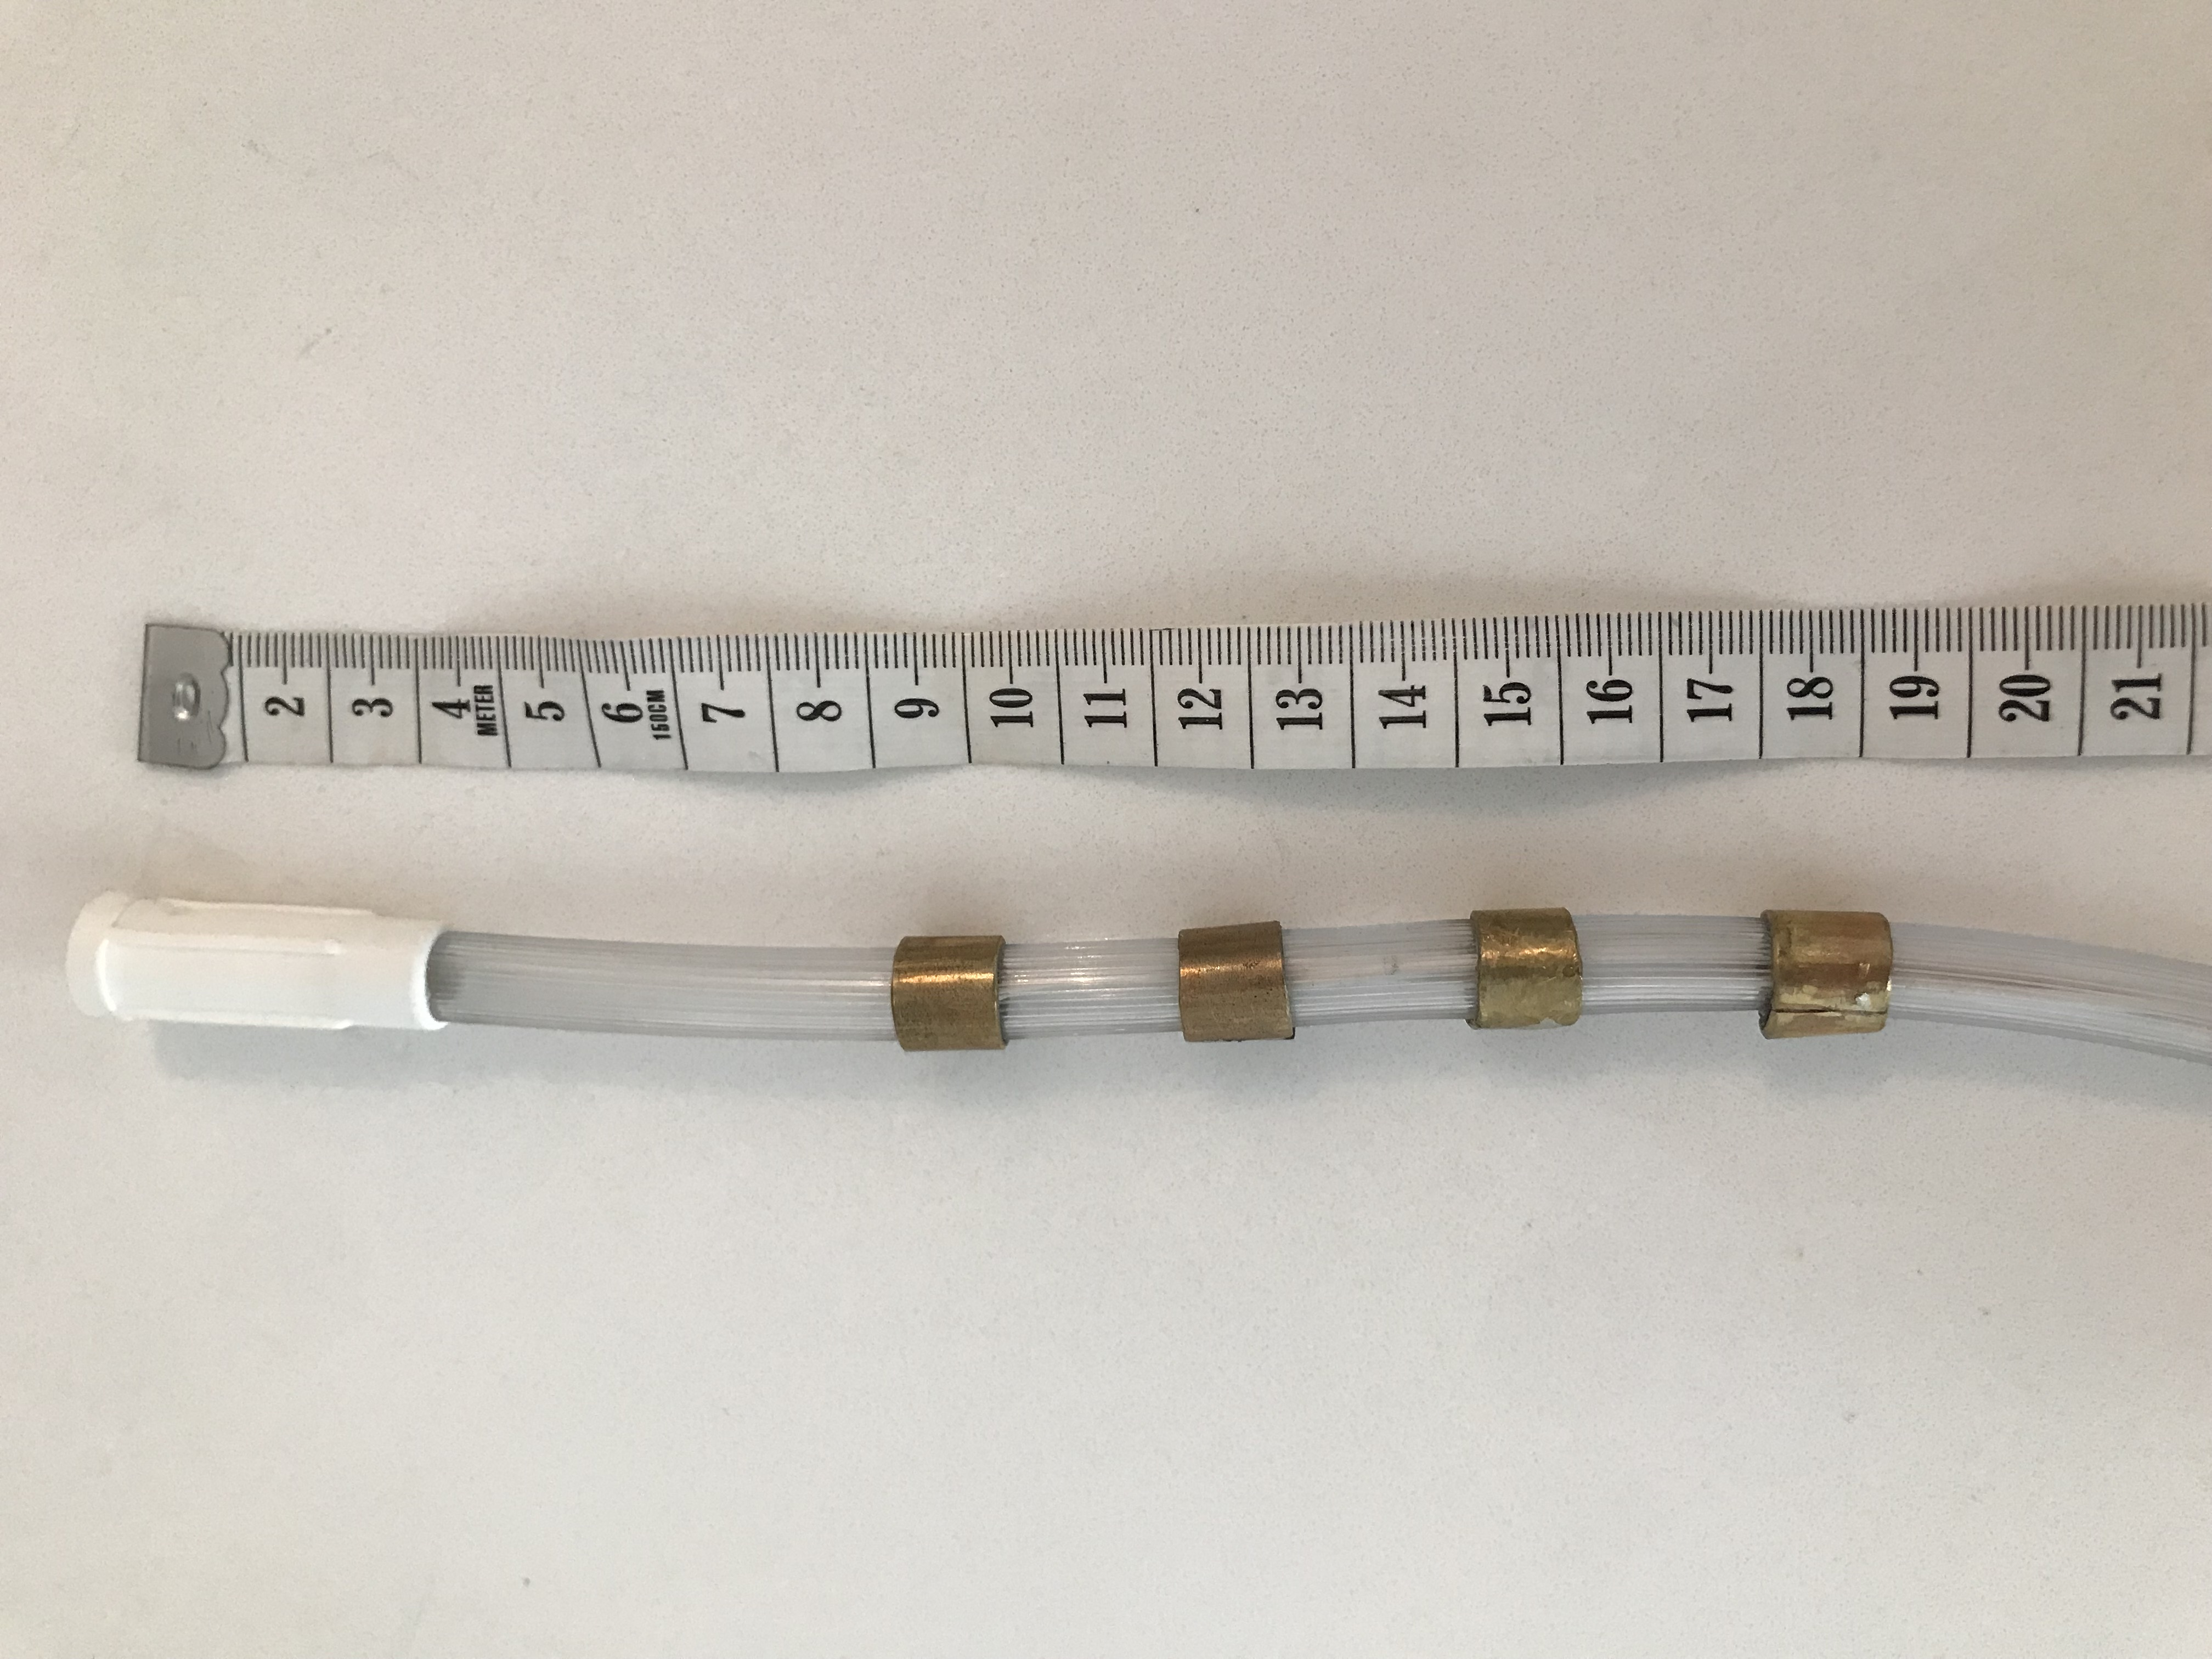
\includegraphics[width=\textwidth, angle =-90]{chapter7-internal_elec_motion/imgs/probe_prototype.jpg} 
	\caption[Probe prototype]{\label{fig:probe_design} 
	A prototype of an internal electrode probe for esophageal use in an ovine model.
	Four brass electrodes are bent around the outside of a flexible tube designed for
	esophageal use. Edges of the electrodes are soldered and filed to be smooth. 
	The electrodes are glued in place and wires run down the hollow centre
	of the tube to connect to the EIT system.}
 \end{figure}

\subsubsection{Electrode placment}
The ewes were shaved and 28 silver-silver chloride electrodes were placed in 2 rows immedeately behind the front
legs with 10 cm seperation and equal spacing around the thorax. 
The esophageal probe was alligned with the electrodes externally and the required
depth was marked. The electrode probe was then coated in a conductive gel for lubraction and inserted in the 
esophagus up to the marked point.

\subsubsection{Ovine Mesh}
An internal probe was added to an ovine mesh by adapting the 
\verb!mk_library_model!
function in EIDORS~\parencite{adler_eidors_2017}. A circular region was added to the
library geometry, and was extruded upwards to make a hole at the probe location. 
The probe was inserted into the mesh just anterior to where the spine would be,
and posterior to the definted lung region. 

The location of the probe in the model relative to lung and heart 
regions is indicated in \fref{fig:ovine_anatomy}. 
\begin{figure}
    \centering
	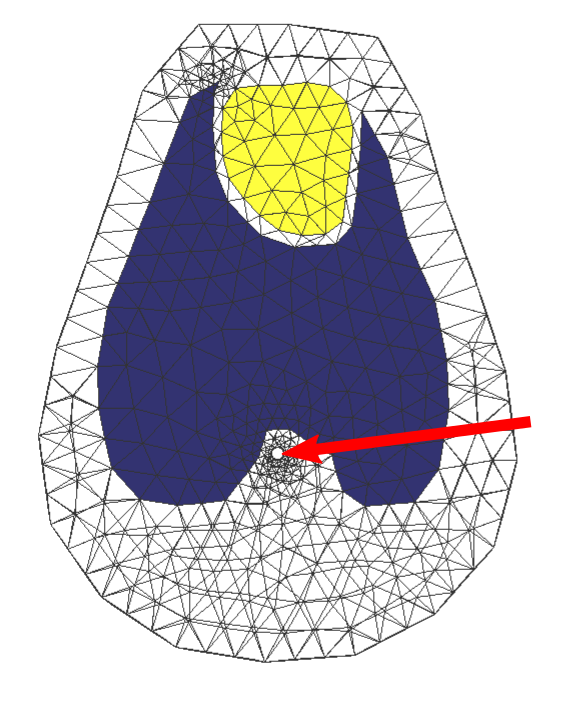
\includegraphics[width=0.95\textwidth]{chapter7-internal_elec_motion/imgs/internal_probe_location.png} 
	\caption[Ovine mesh with organ regions and probe placement]{\label{fig:ovine_anatomy} 
	This figure shows the probe location relative to the lungs and heart. The probe was located 
	at the expected location of the lungs, just anterior to the spine. }
\end{figure}

External electrodes were placed in a square pattern on the boundary, and internal
electrodes were added as cylindrical objects in the central hole of the model.
The resulting model is shown in \fref{fig:internal_lamb_model}.

\begin{figure}
    \centering
	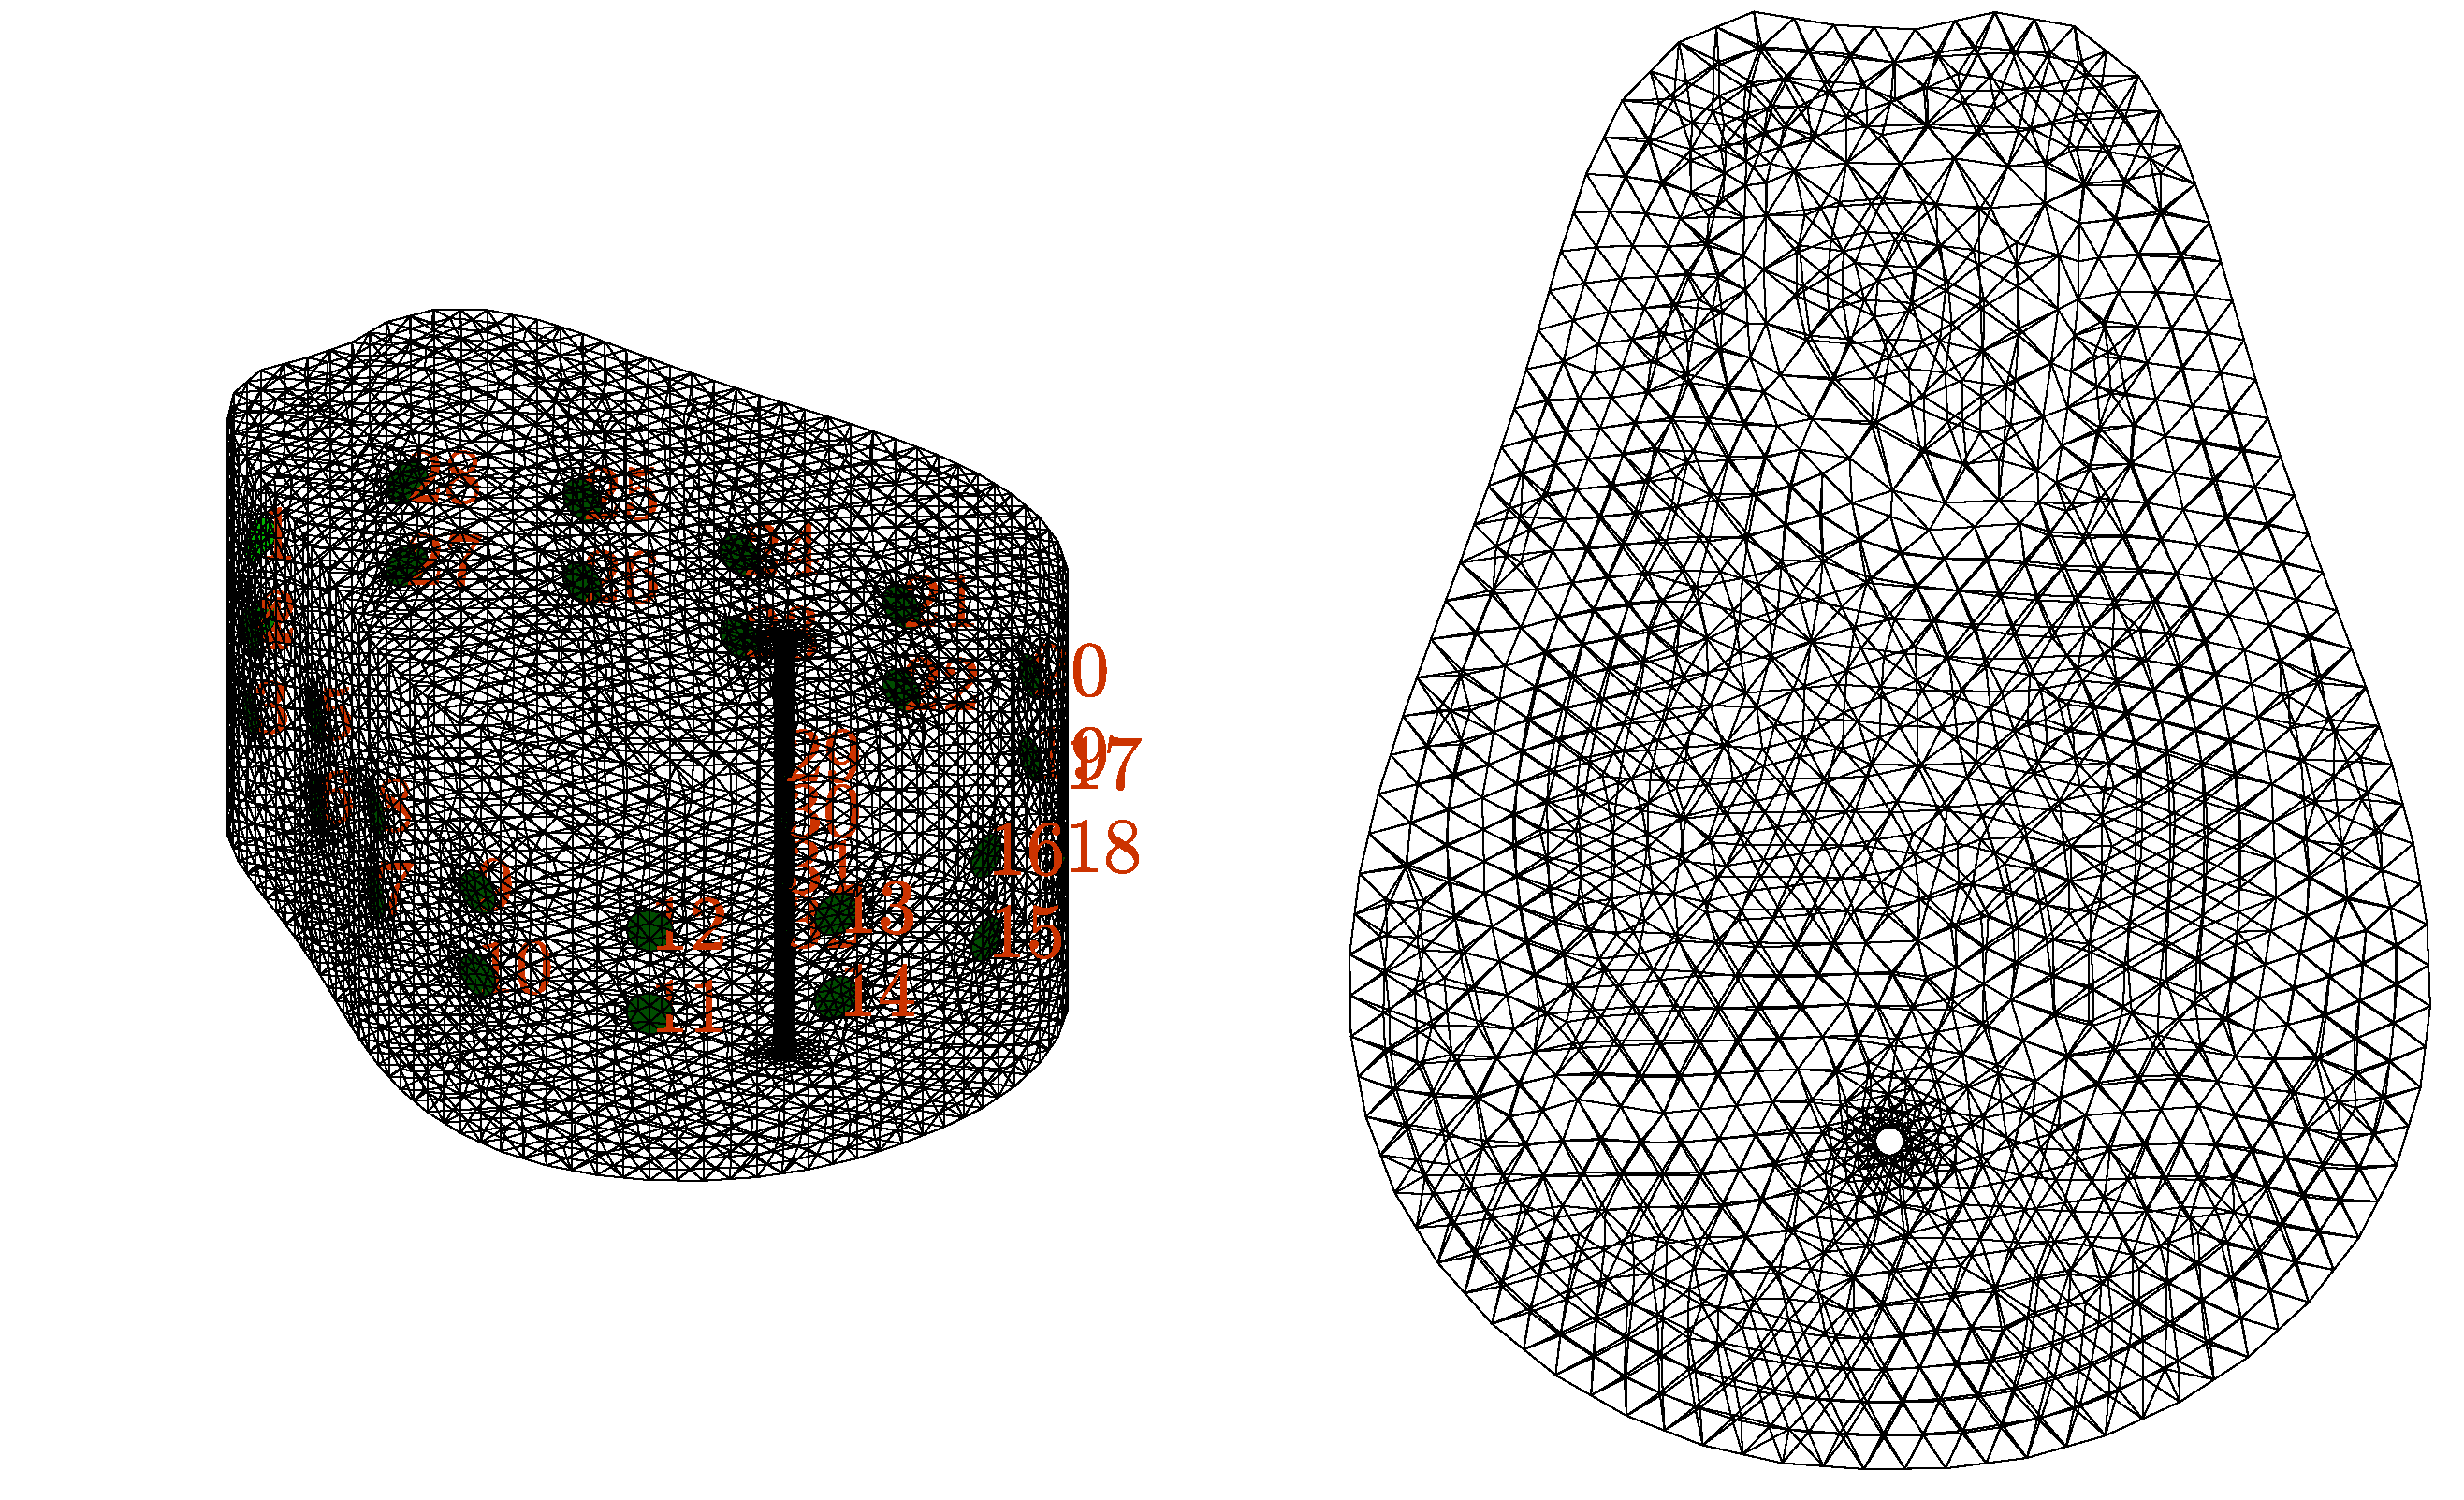
\includegraphics[width=\textwidth]{chapter7-internal_elec_motion/imgs/lamb_model.pdf} 
	\caption[Ovine model with internal probe]{\label{fig:internal_lamb_model} 
	An internal electrode was added to an ovine model by creating a hole at desired probe
	location and added cylindrical electrodes at the desired heights. External electrodes
	were placed in a ``square'' electrode configuration on the boundary. Electrodes 1 to 28 were 
	external and 29 to 32 were internal.}
\end{figure}

\subsubsection{Reconstruction}
To reconstruct images 4 techniques were used. First we compared the 3
techniques in \fref{sec:3_methods}, but GREIT was also used on reconstructions 
of real data.
GREIT for 3D reconstruction has been used with internal electrodes 
\parencite{nasehi_tehrani_evaluation_2012,nasehi_tehrani_modelling_2012}, 
and has been shown to perform well in 3D configurations of external electrodes
\parencite{grychtol_3d_2016}.

To reconstruct images with GREIT 500 training targets with a size of 5 cm were specified, and a noise figure
of 0.5 was used.
images were reconstructed at 10 slices between the electrode planes and summed together to form one 
display image representing the 3D volume.

\subsubsection{Pulsatile amplitude}
The goal of this analysis is to quantify the sensitivity increase with regard to perfusion. 
Although the cardiosynchronous signal may have many sources, we use the 
amplitude of the cardiac-frequency in recorded EIT data as a proxy for sensitivity to 
perfusion related changes. 

To measure the advantage provided by internal electrodes with regard to cardiosynchronous
signal detection, 
a fast Fourier transform (\acrshort{fft}) of each signal was calculated. 
The cardiosynchronous component was selected as the highest 
amplitude near the recorded heart rate range of 65--80 bpm.
This was divided by the amplitude of the ventilation frequency, which was the largest
low-frequency amplitude in the FFT of the detrended signal. 
This was repeated for all 12 recordings across 3 animals.

\section{Results}
The following section presents the results for both simulation and 
\emph{in-vivo} work.

\subsection{Simulation}
When comparing different techniques of modelling internal electrodes, 
it was found that there was no measurable difference between 
simulations of models using spherical internal electrodes 
relative to the
cylindrical electrodes. The results are presented
using the cylindrical model to be consistent with the 
lamb models.
The probe was moved in in the $-\mathbf{y}$ direction for figures and calculations
in the results.

\Fref{fig:probe_location_correction} shows the result of the three reconstruction methods. The boundaries 
of the reconstructed and actual targets are outlined to highlight the performance.
For all rows of the figure the online of the ``true'' conductive region is slightly different. 
This is because when the internal probe is placed in a new location, the entire internal mesh is
slightly different. This resultes in a light change in the number of elecments that are 
in the target region of the model.
All reconstruction techniques were able to reconstruct the object correctly with 1\% 
movement, but there is more blurring and attitive noise in the reconstruction without motion 
correction. With 1\% movement both movement correction techniques are able to accurately 
reconstruct the probe location, but there is a slightly lower level of noise when using the 
new correction technique. 
Ahen the probe is moved by 5\% there is a more pronounced difference between reconstruction 
techniques. When no motion correction is used the amplitude of the artefact is larger than 
the amplitude of the reconstructed image. With basic motino correction the conductive object is
identified correctly, but there is additional noise present in the image. The new techniqe
reconstructs the image accurately and reduces most of the background noise introduced by 
probe movement. 
The new method is the only technique able to reconstruct the correct target location with 
probe motion of 10\% 
of the tank boundary between measurements. The Jaccard index and noise estimate for each method 
are presented below in \fref{tab:recon_accuracy_jaccard} and \fref{tab:recon_accuracy_noise}.

\begin{table}
\centering
\caption[Ovine model with internal probe]{\label{tab:recon_accuracy_jaccard} 
The Jaccard index was calculated for each of the reconstructions in 
\fref{fig:probe_location_correction}. Method A does not use any motion correction.
Method B incorporates the movement jacobian, and method C uses the new probe location correction
technique. For Jaccard index, a score closer to one is better.}
\begin{tabular}{SSSS} \toprule
    {Movement (\% of radius)} & {Method A} & {Method B} & {Method C} \\ \midrule
    1  & 0.732 & 0.809 & 0.802 \\
    5  & 0.038 & 0.654 & 0.808 \\
    10 & 0.003 & 0.000 & 0.577 \\ \bottomrule
\end{tabular}
\end{table}

For movement of 1\% of the tank boundary, motion correction using only the 
movement jacobian was roughly equivalent to the probe location correction algorithm.
Across all other scenarios, the probe location correction  algorithm achieved a higher 
Jaccard score. When intrepreting the Jaccard score, a value of 1 indicates a perfect match
between the actual and reconstructed boundary and a score of 0 indicates that there is no 
overlap between the actual and reconstructed locations.
Across all scenarios the new technique to correct for motion had the lowest 
noise estimate score.
When other techniques were used additional objects were present in the reconstrucionts 
outside of the target objects. When comparing the noise scores, a value closer to 0 is 
better. A value over 1 indicates that the brightest object in the image was not the actual image. 
The way that the noise estimate was calculated always assumed the brightest object was the 
reconstructed image, so no noise score over 1 were recorded.

\begin{table}
	\centering
	\caption[Ovine model with internal probe]{\label{tab:recon_accuracy_noise} 
	Noise estimate values calculated for each of the reconstructions in 
	\fref{fig:probe_location_correction}. Method A does not use any motion correction.
	Method B incorporates the movement jacobian, and method C uses the new probe location correction
	technique. For the noise estimates a lower score is better, a score of zero indicates all image changes
	occur within the target boundary, and a score less than one indicates most of the changes in the 
	image are due to the identified target.}
	\begin{tabular}{SSSS} \toprule
		{Movement (\% of radius)} & {Method A} & {Method B} & {Method C} \\ \midrule
		1  & 0.588 & 0.537 & 0.529 \\
		5  & 0.781 & 0.669 & 0.618 \\
		10 & 0.777 & 0.747 & 0.718 \\ \bottomrule
	\end{tabular}
\end{table}

\begin{figure}
    \centering
	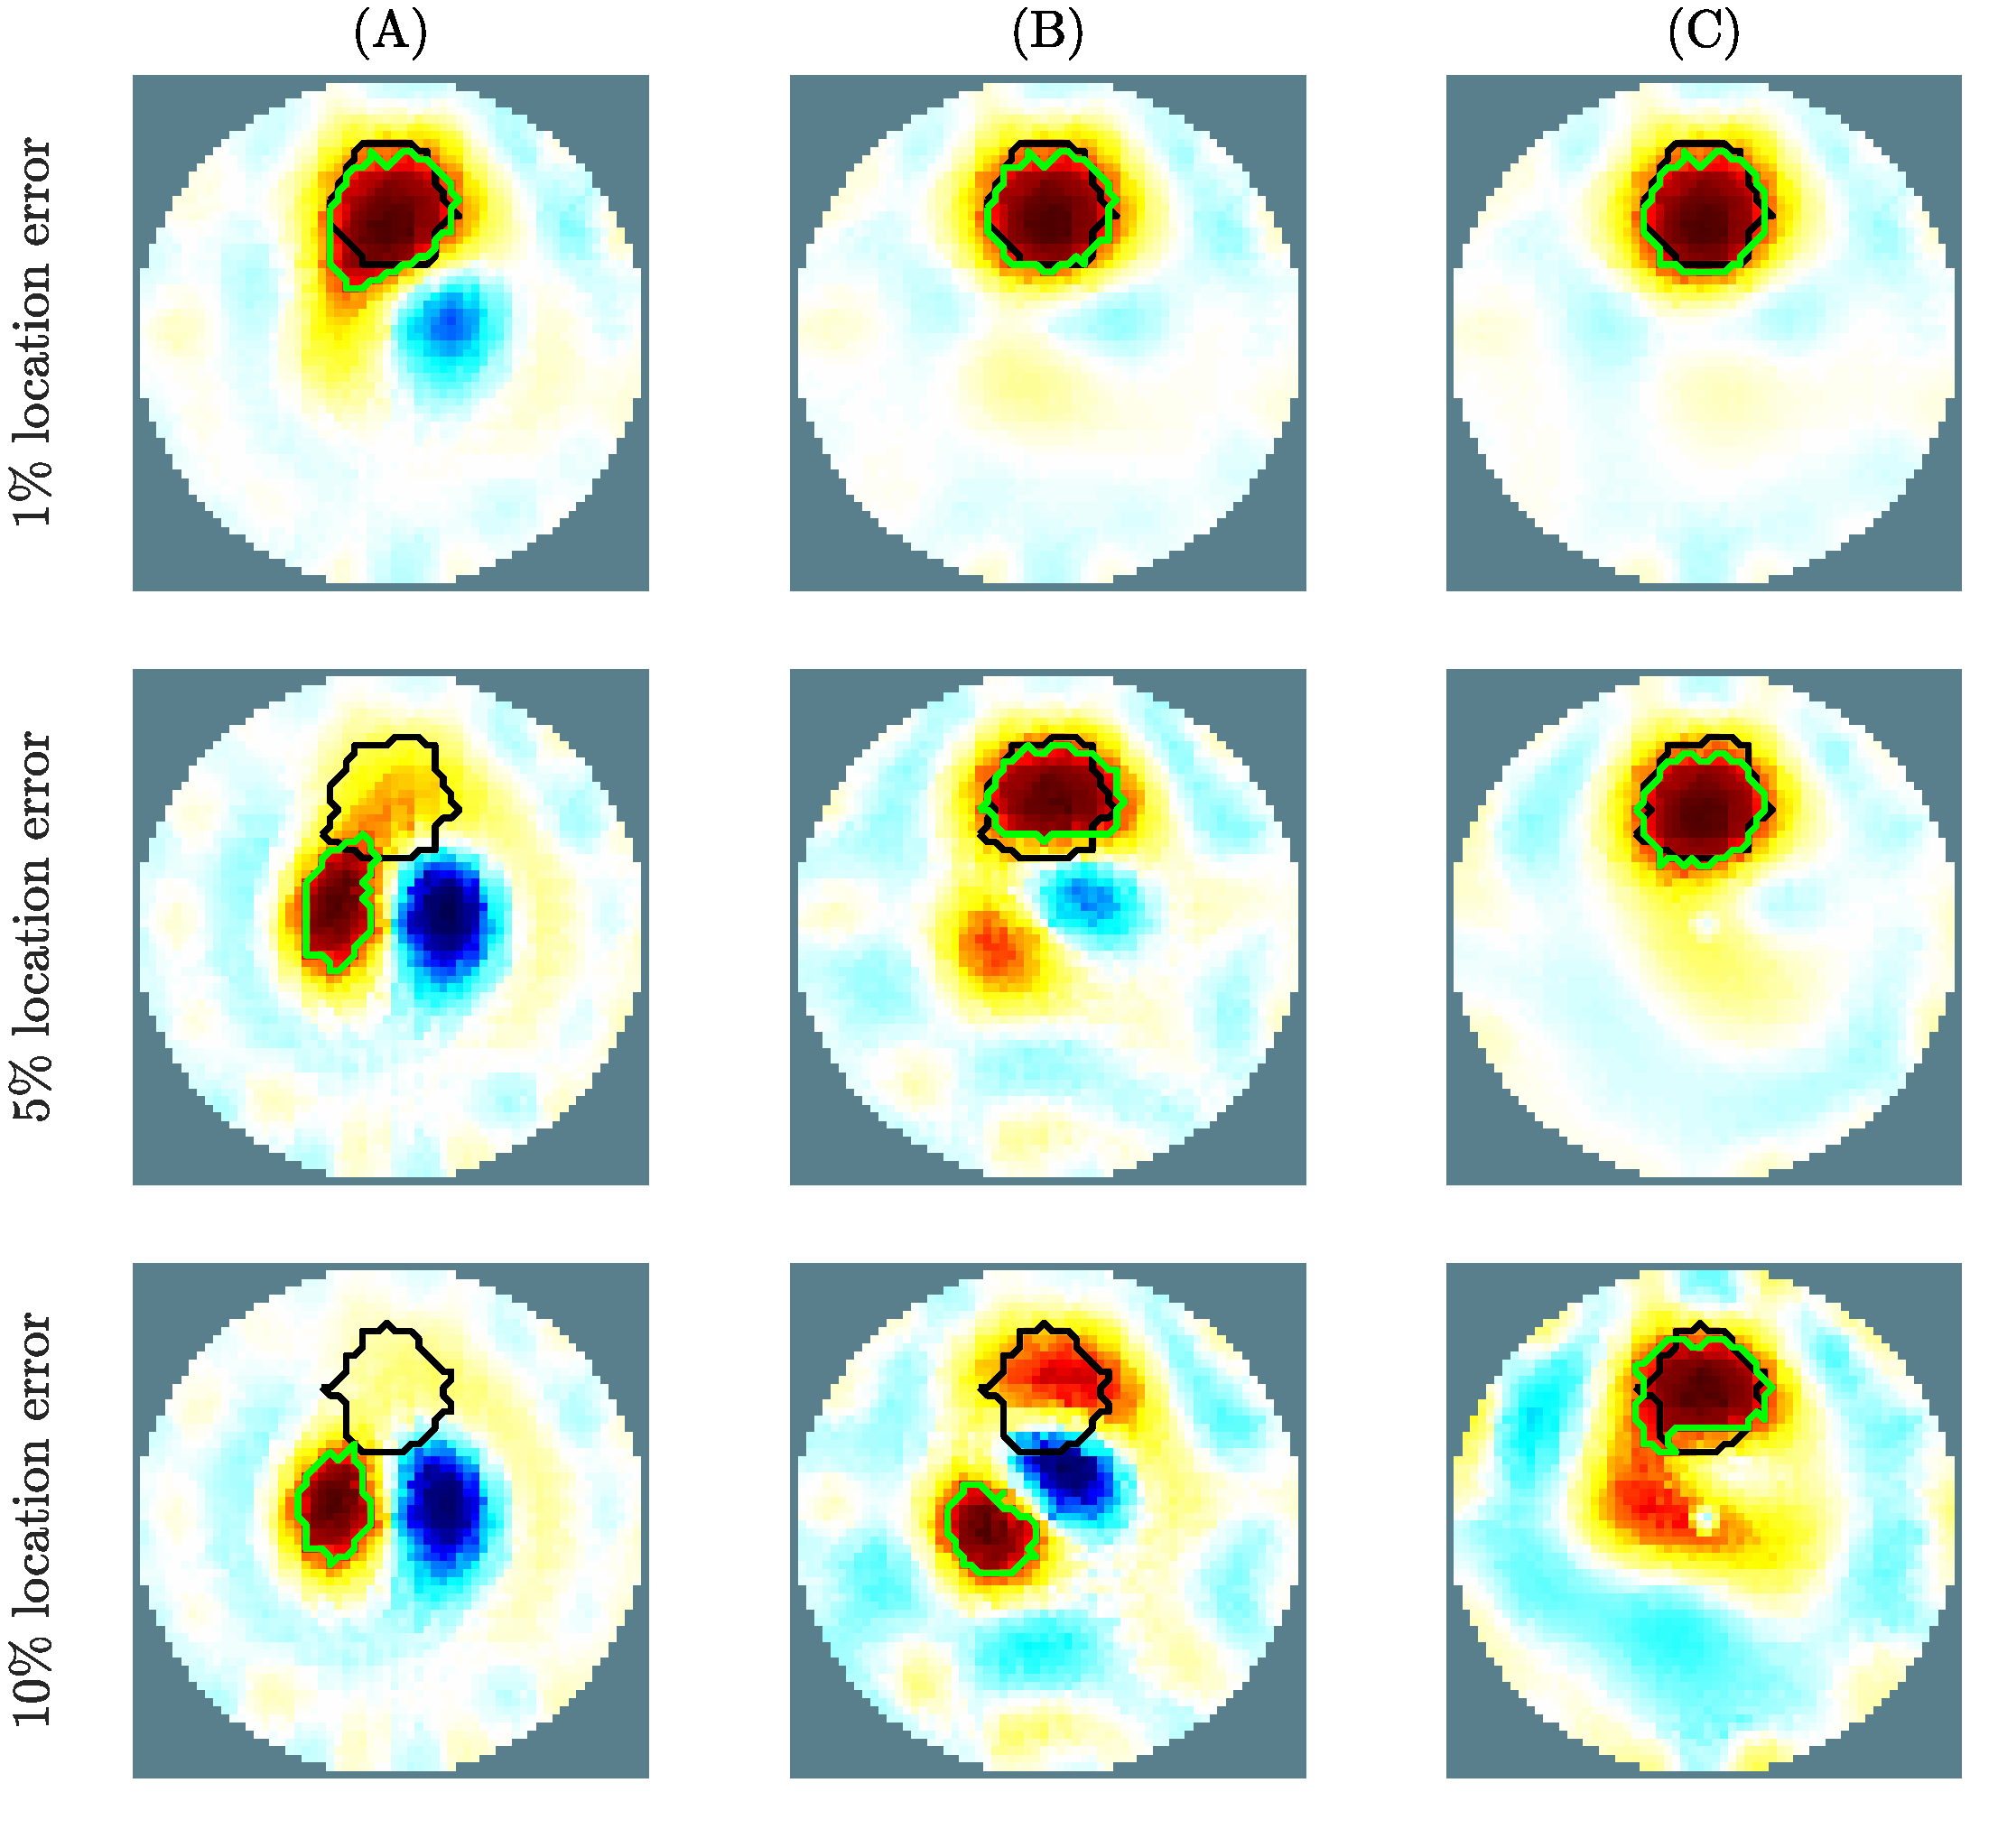
\includegraphics[width=\textwidth]{chapter7-internal_elec_motion/imgs/recon_accuracy_hollow.pdf} 
	\caption[Results of the probe location correction]{\label{fig:probe_location_correction} 
	The results of the probe location correction are presented. 
	The rows from top to bottom show results with 1, 5, and 10\% shifts in probe location 
	relative to the tank radius.
	Column (A) shows the results of the reconstruction  with no motion correction,
	column (B) shows the method using the movement jacobian, and 
	column (C) shows the results of the new probe location correction method.
	The green outline indicates the reconstructed boundary of the conductive target, 
	and the black outline is the actual boundary.}
\end{figure}

When looking at the reconstructions using the three methods, the new probe correction technique
reconstructed the target as the brightest object in all scenarios. With no motion correction, the 
target was identified correctly only in the first scenario. Using the movement jacobaian 
reconstruction method, the target was correctly identified when the probe was moved one or five percent
of the tank radius. 

\subsection{\emph{In-vivo}}
Recordings in each of the three ewes are presented in this section.
Reconstructions with internal electrodes are shown in
\fref{fig:internal_reconstructions} for a selected breath during a 
baseline recording in each subject.

\begin{figure}
    \centering
	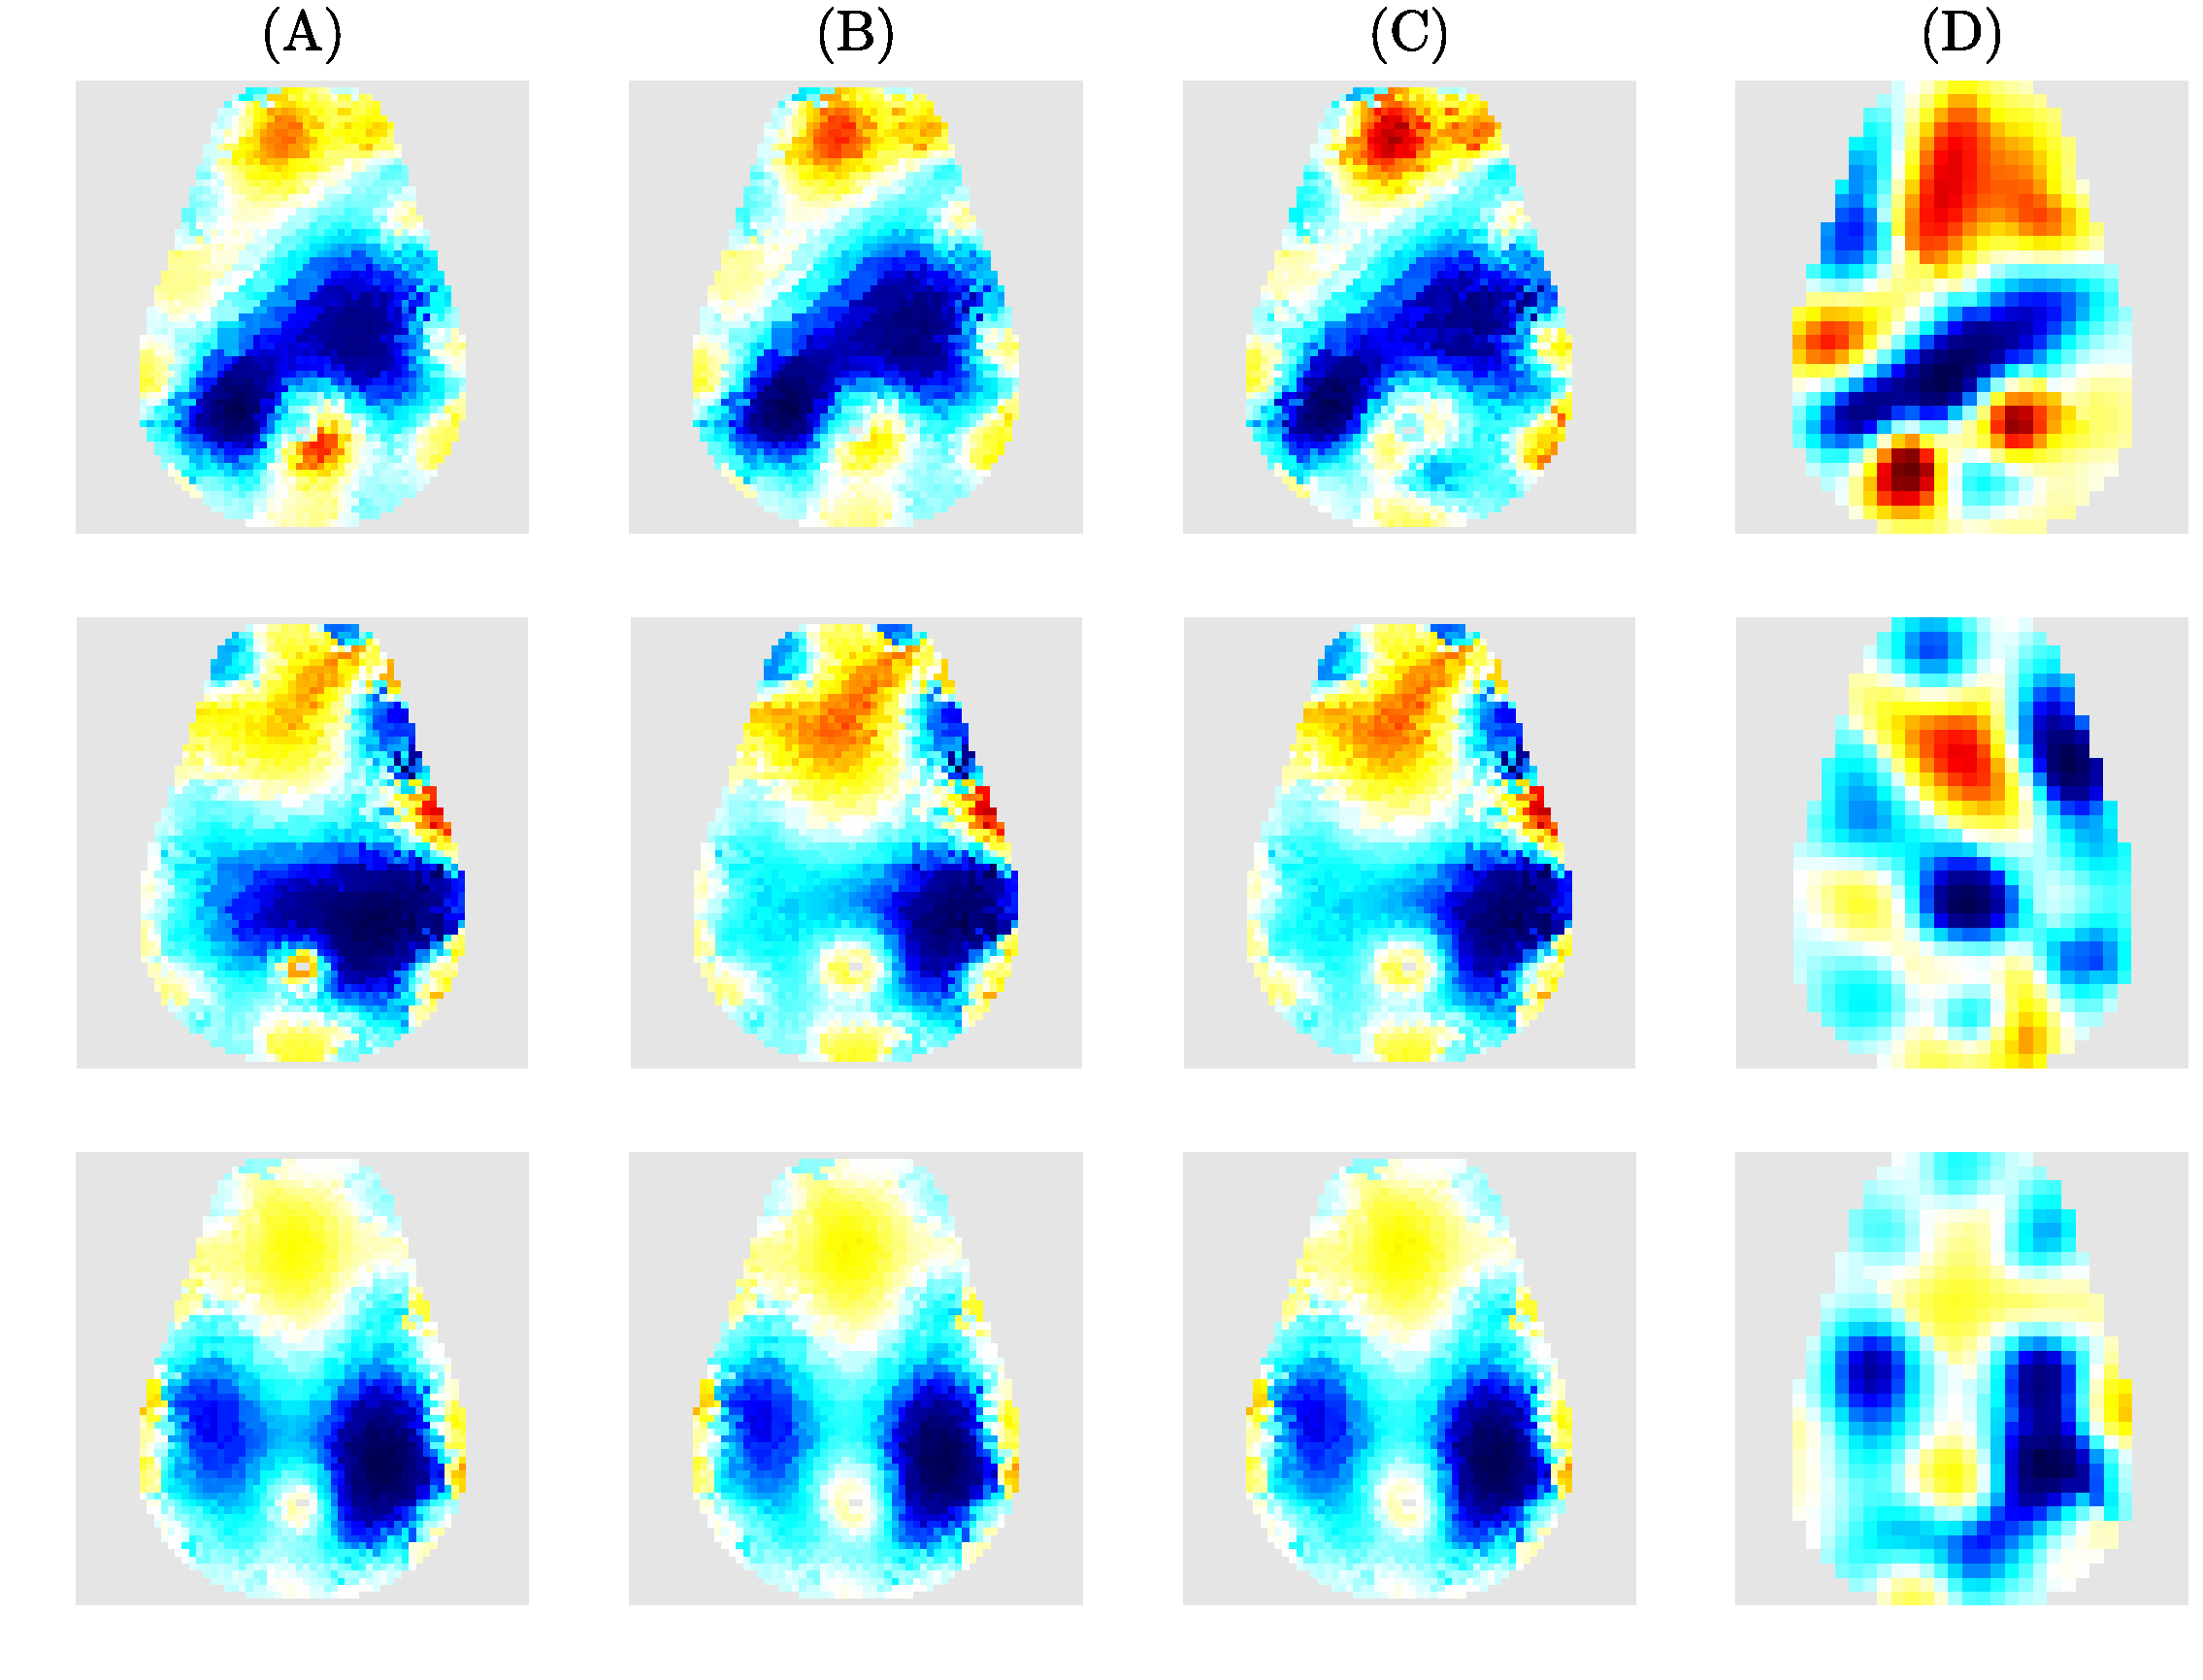
\includegraphics[width=\textwidth]{chapter7-internal_elec_motion/imgs/lamb_reconstruction_all.pdf} 
	\caption[Results of the probe location correction]{\label{fig:internal_reconstructions} 
	Preliminary results on 3 ewes reconstructed 
	from a single, selected breath. Each column represents a reconstruction method. Column (A)
	uses no motion correction, column (B) uses the movement jacobian and column (C) uses the new method
	for electrode location correction. Column (D) contains reconstructions using the GREIT 3D algorithm.
	The number of pixels is different between images due to the methodology of probe localization and 
	the limitations of GREIT.}
\end{figure}

Reconstructions with movement correction applied to the internal electrodes appear to show a 
slight improvement in lung distinguishability and a slight reduction
in noise surrounding the probe. There is limited difference between the
two methods accounting for motion on the electrode.

The ratio of cardiosynchronous to respiratory rate impedance signals is shown below in 
\fref{fig:amplitude_ratio}. The results show a higher amplitude of the cardiopulmonary 
signal relative to ventilation when internal electrodes are used.

\begin{figure}
    \centering
	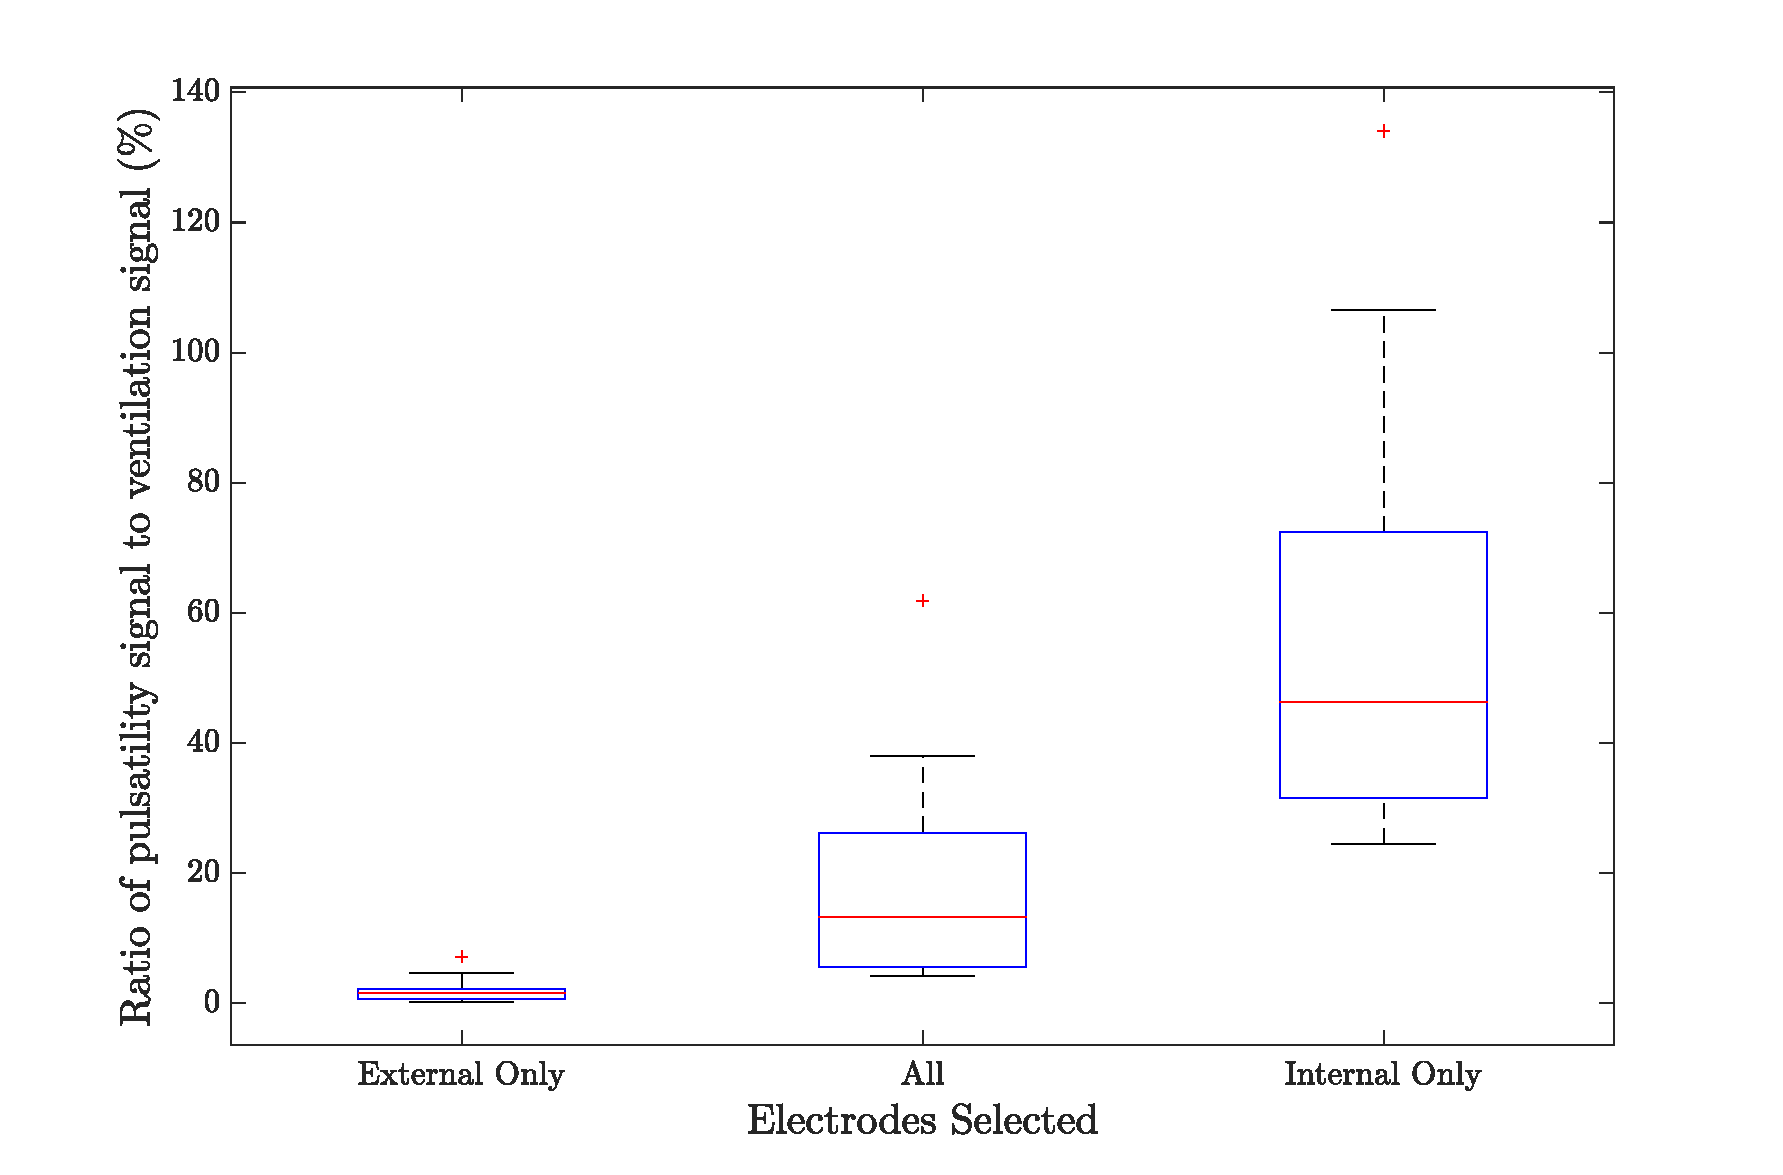
\includegraphics[width=\textwidth]{chapter7-internal_elec_motion/imgs/amplitude_ratio.pdf} 
	\caption[Results of the probe location correction]{\label{fig:amplitude_ratio} 
	The cardiosynchronous signal component was divided by the ventilation frequency 
	componenent to compare the detectability of the pulsatile changes. The ratio was compared 
	for measuremnts using only external electrodes, all electrodes, and internal electrodes only.}
\end{figure}~

\section{Discussion}

This chapter aimed to provide a technique to reduce noise due to motion on internal
electrodes when reconstructing images in 3D and demonstrate the noise reduction technique
\emph{in-vivo}. The new technique to reconstruct images in the presence of motion 
on internal electrodes reconstructed an image of a conductive target 
more accurately and with less noise in the surrounding image. \emph{In-vivo}
reconstructions showed a slight improvement in lung distinguishability when correcting
for motion artefacts on internal electrodes compared to methods without this correction 
including GREIT. Results in 3D also aligned with results from a 2D study in a porcine 
model showing an increased cardiosynchronous component on the internal electrode 
measurements~\parencite{czaplik_application_2014}.

It was found that GREIT performed poorly when reconstructing data with internal electrodes.
The figures of merit for GREIT were designed and optimized to work with external electrodes 
where sensitivity is low in the centre of the model and high at the 
edges~\parencite{adler_greit_2009}. An adaptation to GREIT that is able to 
account for internal electrodes and motion of an internal probe is planned as a
continuation of this project.  

Two types of internal electrodes were modelled in this chapter. One with
spherical internal electrodes and one with a hollow probe and cylindrical electrodes. 
Meshing and creating internal electrodes can be challenging due to limited meshing tools 
for using internal electrodes with EIT and the method of adding internal probes to
anatomical models using a hollow region in the centre of the model was created for this 
project. Code to generate this model with internal electrodes is planned to be included in a
future release of EIDORS.

The noise estimate score calculations were not perfect representations of the noise
in the images due to the way the reconstructed object was identified.  Since the
brightest object was always identified as the object, the noise estimate was
artificially low in some cases. 
Comparing the amplitude of changes contained within the true
object boundaries could be a better metric of the noise present in the image, but this
would also be dependent on the accuracy of reconstruction and would have favoured
the method that reconstructed the object most accurately.
The boundary of the true target
also changes due to differences in element locations as the 
probe is moved, so the comparison would not be consistent across all probe movement
states. Despite this limitation, the noise estimate does help to quantify 
noise seen in the images for each technique. 
The new
method performed better than existing techniques across all situations according to the computed
noise metrics.

In simulated cases of less than one percent error in probe location, very little 
difference in reconstruction accuracy between 
the two motion correction algorithms was detected. 
Despite this, a slight reduction 
in background noise in the image was observed. 

Despite the improvements to reconstruction accuracy 
and noise reduction using the new method, there are several limitations to its use. 
The largest is 
the increased modelling time required. This method required an extra model, and inverse 
solution compared to the single step solutions. For simple models such as 
a tank the added time difference
is small, but for complex models this could increase reconstruction time drastically. 
When several frames are reconstructed each requires a unique model 
with a modified probe location increasing the time required. 
To reduce the reconstruction 
time, correcting the model only when the  probe location error is greater than one 
percent of the model radius may be helpful. At this 
level of movement, the benefits of 
the probe localization technique are 
not substantial. 
Additionally in the images presented probe movment did not 
appear to be large. It is not yet clear what the typical movement of the electrode probe 
is expected to be in the esophagus. 

Previous research has also 
reconstructed for motion direction directly using the movement
jacobian~\parencite{boyle_geophysical_2016,gomez-laberge_direct_2008,soleimani_imaging_2006}.
This technique for electrode estimation has not been implemented using internal electrodes 
for this research, but a comparison between the two electrode position estimation techniques 
it required for complete validation of the demonstrated method.

Previous studies with internal electrodes showed cases where contact impedance of the probe
was inadequate for electrodes
placed on the breathing and feeding tubes~\parencite{czaplik_application_2014}.
The electrodes used were shown to have a good contact impedance on the SenTec Pioneer
Set interface, but the current design protrudes slightly from the tube and may be challenging to 
integrate into a clinical esophageal or tracheal tube.

\citeauthorandyear{sanchez_vivo_2013} used an array of internal electrodes in the lung 
during biopsy procedures, and suggested that the increased proximity to the 
tissue could allow more physiological information to be obtained. A more complete 
evaluation is required to measure the benefits of internal electrodes in 3D compared 
to typical external configurations. The previously seen lung distinguishability
and larger cardiosynchronous signal amplitude found in 2D~\parencite{czaplik_application_2014} 
have been repeated with this 3D configuration, but it is still unclear to what 
degree these signal changes may be useful. 

Increased lung separability may be useful for determining the difference between right 
and left lung ventilation, which can be used to quantify ventilation 
performance~\parencite{sage_assessing_2018}
and is an important step in detecting ventilation and perfusion
mismatch~\parencite{stowe_comparison_2019,kircher_regional_2021,leonhardt_electrical_2012}.
Increased sensitivity to pulsatile flow may also help to improve measures
of cardiopulmonary activity where detecting pulsatile flow 
and motion in specific regions of a model is 
desired~\parencite{braun_accuracy_2018,proenca_non-invasive_2020}.

\section{Summary}
Probe displacement introduces large errors when using 
reconstruction algorithms that do not account for movement. This chapter presents
a new technique designed to reduce the effect of probe motion.
This new method 
was found to outperform existing methods with regards to reconstruction 
accuracy and background noise in simulations on a tank model. 
Internal electrodes in conjunction with a 3D external configuration were also 
used \emph{in-vivo} to measure ventilation. 
Images of breaths across three subjects showed an improvement to lung distinguishability
when correcting for motion, and the average ratio of cardiosynchronous
to pulmonary signal was increased when using internal electrodes. 